\section{Regression}
We have chosen to predict the attribute : "2-Hour serum insulin concentration"
because we found out in the last report that this attribute had a great influence on the dataset.
It is therefore of our greatest interest to solve this problem.

\subsection{Linear regression}

\subsection{Artificial Neural Network}

\subsection{Model comparison}


\section{Classification}

This data set contains an obvious binary attribute
with clinical relevance:
does the patient have diabetes or not?
As such, this question is what we will be
focusing our classification efforts on.

\subsection{Decision tree}
Decision trees are a way to split your training data into subsets. These splits are based on that attribute's value.
These subsets can then predict the datapoint's class.
One of three models we have chosen to adress our classification problem with is the
decision tree. Decisions trees with the capacity to classify observations are called
classification trees. These trees sort the data by using Hunt's algorithm, which
splits the tree iteratively, and for each iteration keeps the split with the
highest purity gain. For this decisions tree, the "gini" impurity gain has been
chosen to quantify impurity gain. The algorithm can be stopped, and has indeed
been done so here, both by providing a maximum "depth" (or number of iterations
of splits) or by providing a minimum number of number of samples at a given
place in the tree to keep trying to improve the impurity.
The inner loop of a doubble-layered cross-validation for the decision tree
(which consisted of a leave-one-out cross-validation) showed
that the model is quite robust with regard to the tree-depth, which performed
best at the value of 3, given the following tree (when taken on all the available
data):

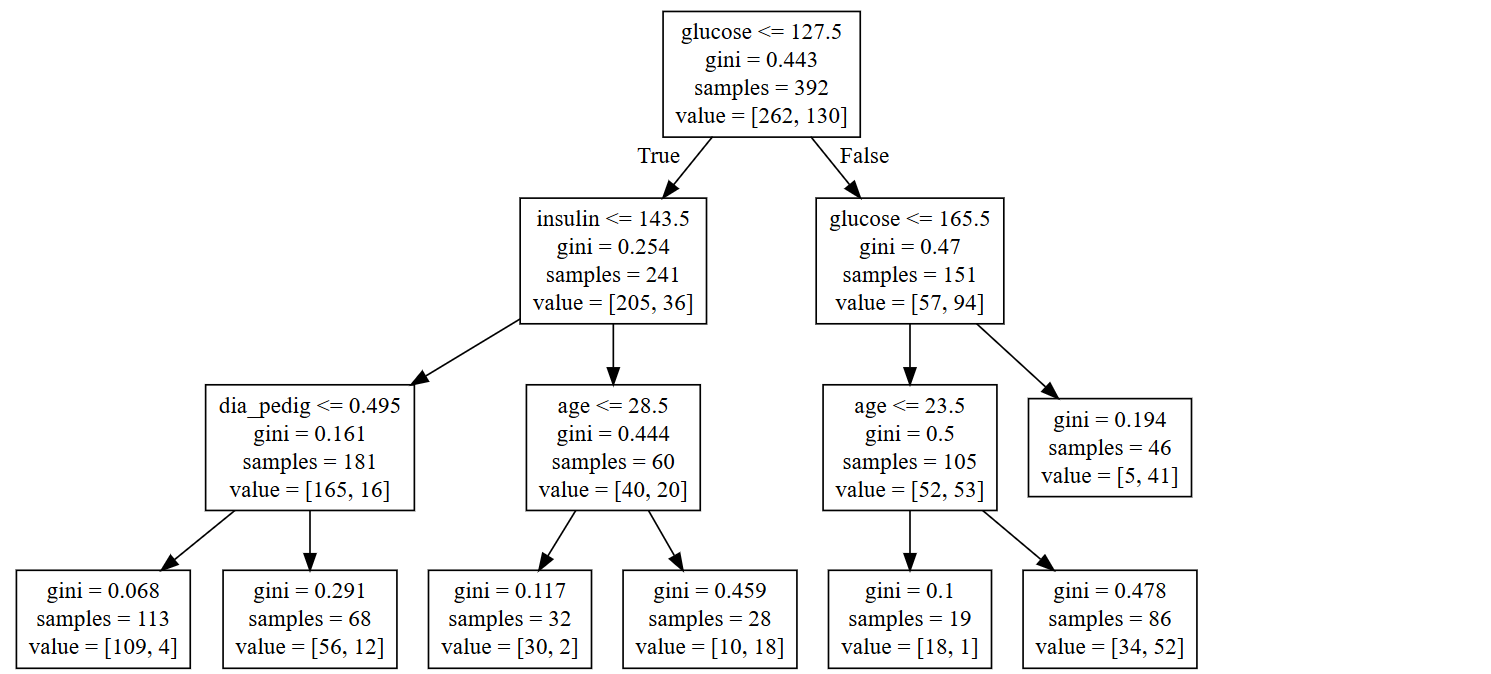
\includegraphics[width=\textwidth]{tree.png}

So, when given a datapoint, the first thing to do when using the tree to figure
out whether to classify a patient as with or without diabetes, is to ask whether
the patient's glucose level is equal to or below 127.5. If true, the insulin level
accounts for the next split, and if false, glucose once more, but with another
value this time, accounts for the split. Which box an observation or patient belongs
to in the last tier determines whether or not we believe the patient to have diabetes
or not.

\subsection{$k$-nearest neighbours}
The KNN-method takes a datapoints' K-amount of nearest neighbours and learns to predict the datapoints' class.
This is done by using the leave-one-out method and letting the model test the it's own ability to predict the classes.
The method is then repeated with a higher amount of neighbours and the test-error is then found.
The second model used is a $k$-nearest neighbors model. In our model, the nearest
neighbour will be the neighbour with the shortest euclidean distance to the observation.
This may become troublesome in higher-dimensional data, but with our 8 attributes, it should
not be too bad. The best number of neighbours were found in the inner loop with
the leave-one-out method, however, the best k's seem to change quite a bit for the
different data feeded to this loop by the outer loop, as can be seen below in the performance
tables. The best performing k can be seen to be 19, however, another k was
28 in the same run! This means that the parameter k for the model is not very
robust and is prone to change a lot. When the k has been chosen, the model then
predicts an observation's class based on its k nearest neighbours (as the
name suggests). This means that if the best performing k is 19, and the 10
data points that are closest to it by the euclidean distance is a given class,
then this class is chosen as the predicted class. This is hard to visualize
graphically because the dimension of our data is more than 3. Overall, this
method seems to perform similarly to the tree model.

\subsection{Artificial Neural Network}
The ANN model is the last model chosen to classify with. Results??

\subsection{Logistic regression and Naive Bayes}
Logistic/Multinomial Regression:
Is a way to try to predict the probability of the datapoint being from a certain class,
based on linear regression.
The method is similar to linear regression, except we can make a general linear model in which we make a great set of linear regression
and thereafter find the probability of that attribute of being in a certain class.
Naive Bayes:
This method can predict a datapoint's class from its' position and the probability
of being in the either one of the classes. It does this by comparing the already existing
datapoints' positions and then calculates the probability of a new datapoint being in that
class depending on it's value.


Articial Neural Networks (ANN):
MARCUS !!!!!!! hjælp, jeg forstår det ikke ):



\subsection{Model comparison}
We compared the ANN and the decision tree. We did this through finding their difference in accuracy rate.
The classifiers are seen as different if their accuracy rate is significantly different from zero. The better one being
the classifier being better at predicting correctly.

\begin{table}[]
\centering
\caption{My caption}
\label{my-label}
\begin{tabular}{@{}lllll@{}}
\toprule
fold                                                                      & KNN  & ANN  & Trees &  \\ \midrule
\multicolumn{1}{|l|}{\cellcolor[HTML]{34FF34}{\color[HTML]{000000} 1}}    & 0.78 & 0.72 & 0.80  &  \\ \cmidrule(r){1-1}
\multicolumn{1}{|l|}{\cellcolor[HTML]{34FF34}{\color[HTML]{000000} 2}}    & 0.75 & 0.59 & 0.70  &  \\ \cmidrule(r){1-1}
\multicolumn{1}{|l|}{\cellcolor[HTML]{34FF34}{\color[HTML]{000000} 3}}    & 0.71 & 0.67 & 0.71  &  \\ \cmidrule(r){1-1}
\multicolumn{1}{|l|}{\cellcolor[HTML]{34FF34}{\color[HTML]{000000} 4}}    & 0.78 & 0.79 & 0.74  &  \\ \cmidrule(r){1-1}
\multicolumn{1}{|l|}{\cellcolor[HTML]{34FF34}{\color[HTML]{000000} 5}}    & 0.77 & 0.67 & 0.77  &  \\ \cmidrule(r){1-1}
\multicolumn{1}{|l|}{\cellcolor[HTML]{FFFFFF}{\color[HTML]{000000} mean}} & 0.76 & 0.69 & 0.74  &  \\ \cmidrule(r){1-1}
\multicolumn{1}{|l|}{\cellcolor[HTML]{FFFFFF}{\color[HTML]{000000} std}}  & 0.03 & 0.07 & 0.04  &  \\ \bottomrule
\end{tabular}
\end{table}

\section{Previous work}

\appendix
\section{Distribution of responsibilities}
